\documentclass[12pt,a4paper]{article}
\usepackage[warn]{mathtext}
\usepackage[utf8]{inputenc}
\usepackage[T2A]{fontenc}
\usepackage[english,russian]{babel}
\usepackage{indentfirst}
\usepackage{misccorr}
\usepackage{subcaption}
\captionsetup{compatibility=false}
\usepackage{geometry}
\geometry{verbose,a4paper,tmargin=2cm,bmargin=2cm,lmargin=1.5cm,rmargin=1.5cm}
\usepackage{graphicx}
\usepackage{wrapfig}
\usepackage{amsmath}
\usepackage{floatflt}
\usepackage{float}
\usepackage{amssymb}
\usepackage{color}
\usepackage{lscape}
\usepackage{hvfloat}
\usepackage{amsfonts}
\usepackage{euscript}


\graphicspath{ {images/} }
\usepackage{multicol}
\setlength{\columnsep}{2cm}


\begin{document}

\begin{titlepage}
	\centering
	\vspace{5cm}
	{\scshape\LARGE Московский физико-технический институт \par}
	\vspace{5cm}

	{\huge Лабораторная работа № 4.1.2 \par}
	\vspace{1cm}
	{\scshape\Large "Моделирование оптических приборов и определение из увеличения"\par}
	\vspace{2cm}
	\vfill
\begin{flushright}
	{\Large Выполнила студентка Б01-903}\par
	\vspace{0.3cm}
	{\LARGE Юлия Прохорова} \par

	
\end{flushright}
	

	\vfill\large

% Bottom of the page
	Долгопрудный, 2021 г.
\end{titlepage}

\section{Цель работы:}
Определить фокусные расстояния собирающих и рассеивающих линз, смоделировать ход лучей в трубе Галилея, 
трубе Кеплера и микроскопе, определить их увеличение.

\section{Оборудование:}
Оптичесая скамья, набор линз, экран, осветитель со шкалой, зрительная труба, диарагма, линейка.

\section{Теоретическая часть}

В работе изучаются модели зрительных труб и микроскопа, которые состоят из объектива - линзы,обращенной
 к объекту, и окуляра - линзы, обращенной к наблюдателю.

\begin{figure}[h]
    \begin{center}
    \begin{minipage}[h]{0.4\linewidth}
    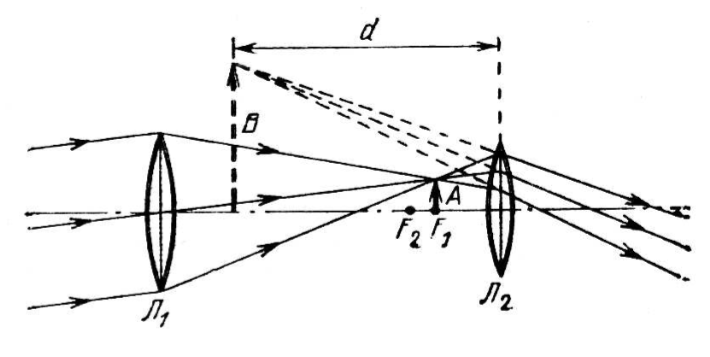
\includegraphics[width=1\linewidth]{kepler.png}
    \caption{Ход лучей в трубе Кеплера}
    \label{kepler}
    \end{minipage}
    \hfill
    \begin{minipage}[h]{0.45\linewidth}
    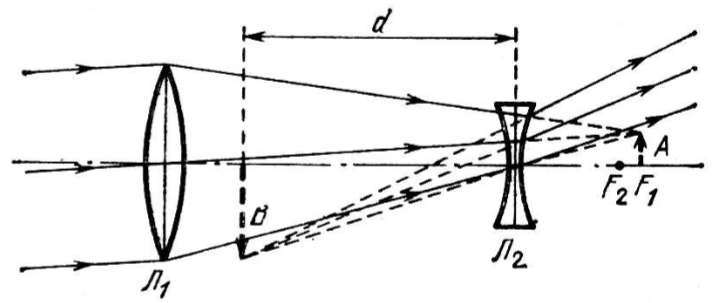
\includegraphics[width=1\linewidth]{galiley.png}
    \caption{Ход лучей в трубе Галилея}
    \label{galiley}
    \end{minipage}
    \end{center}
\end{figure}

\begin{figure}[H]
    \begin{center}
    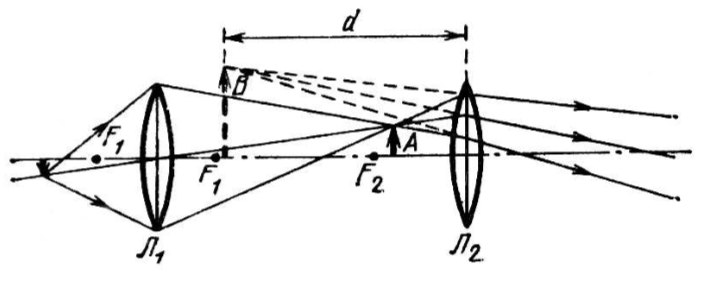
\includegraphics[width=8cm]{microscop.png}
    \caption{ Ход лучей в микроскопе}
    \label{micro} %% метка рисунка для ссылки на него
    \end{center}
\end{figure}

В случае зрительных труб, предназначенных для наблюдения за удаленными (расстояние значительно превышает фокусное расстояние) объектами, изображение А предмета находится практически в факальной плоскости.
В случае же микроскопа  - промежуточное изображние А находится далеко за фокальной плоскостью объектива.
\par
Мнимое же изображение B, даваемое окуляром, располагается на расстоянии d от окуляра.
\par
\textit{Отношение углового размера изображения объекта, рассматриваемого невооруженным 
глазом, называется угловым увеличением оптического прибора.} 
\par
\textbf{Увеличение астрономической зрительной трубы (трубы Кеплера).}  Задний фокус объектива совпадает
с передним фокусом окуляра. В этом случае труба  - \textit{афокальная система}: параллельный пучок лучей, входящих в объектив, остается параллелльным по выходе
из окуляра. Такой ход лучей - \textit{телескопический}.

\begin{figure}[H]
    \begin{center}
    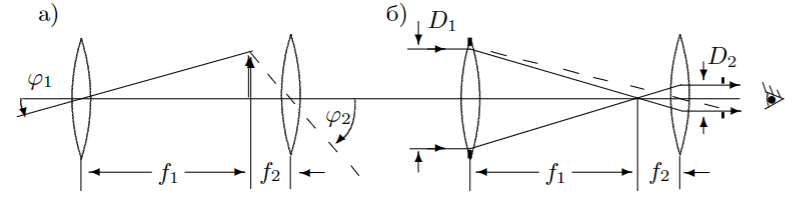
\includegraphics[width=10cm]{uvelichenie_1.png}
    \caption{ К расчету увеличения зрительной трубы Кеплера}
    \label{uvelichenie_1} %% метка рисунка для ссылки на него
    \end{center}
\end{figure}

Пусть пучок света, попадающий в объектив, составляет с оптической осью угол $\varphi_1$, а пучок, выходящий из окуляра, - $\varphi_2$, тогда увеличение $\gamma$ зрительной трубы:
\begin{equation}
    \gamma = \frac{tg\varphi_2}{tg\varphi_1} = \frac{f_1}{f_2}, \label{eq:gamma_1}
\end{equation}

$\varphi_1$ - угловой размер объекта, а при наблюдении бесконечно удаленного объекта и для объектива, и для глаза он одинаков.

Отношение фокусных расстояний равно отношению диаметров пучка, отсюда:

\begin{equation}
    \gamma = \frac{D_1}{D_2}, \label{eq:gamma_2}
\end{equation}
Когда $D_2$ равен диаметру $d_0$ зрачка наблюдателя, увеличение  - \textit{нормальное}.

\par
\textbf{Увеличение гаилеевой зрительной трубы.} При телескопическом ходе лучей расстояние между объективом и окуляром равно разности
их фокусных расстояний.

\begin{figure}[H]
    \begin{center}
    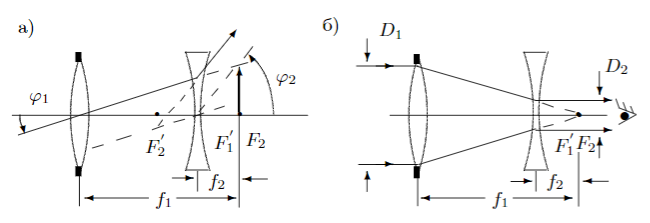
\includegraphics[width=10cm]{uvelichenie_2.png}
    \caption{ К расчету увеличения галилеевой зрительной трубы}
    \label{uvelichenie_2} %% метка рисунка для ссылки на него
    \end{center}
\end{figure}

Формулы \ref{eq:gamma_1} и \ref{eq:gamma_2} справедливы и для земной. Достоинство такой труб - прямое изображение.

\textbf{Увеличение микроскопа.} 

\begin{figure}[H]
    \begin{center}
    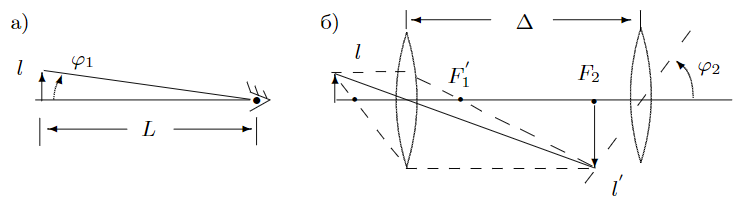
\includegraphics[width=10cm]{uvelichenie_3.png}
    \caption{ К расчету увеличения микроскопа}
    \label{uvelichenie_3} %% метка рисунка для ссылки на него
    \end{center}
\end{figure}

Тангенс угла $\varphi_2$, под которым видно изображение, определяется соотношением:
\begin{equation}
    tg\varphi_2 = \frac{l'}{f_2} = \frac{l(\Delta - f_1 - f_2)}{f_1f_2} \label{eq:tg}
\end{equation}
где $l'$ - размер промежуточного изображения, l - размер предмета, $\Delta$ - длина тубуса (расстояние между линзами).
\par
Угловой размер предмета l:
\begin{equation}
    tg\varphi_1 = \frac{l}{L} \label{eq:tg_2}
\end{equation}

\par
Увеличение микроскопа:
\begin{equation}
    \gamma = \frac{tg\varphi_2}{tg\varphi_1} = \frac{L(\Delta - f_1 - f_2)}{f1f2} \label{eq:gamma_3}
\end{equation}

Можно показать, что при аккомодации глаза на L угловое увеличениеравно линейгому Г:
\begin{equation}
    \gamma = \frac{tg\varphi_2}{tg\varphi_1} = \frac{L(l''/L)}{l/L} = \frac{l''}{l} = Г \label{eq:Gamma}
\end{equation}
где l'' - рамер окончательного изображения.

\begin{equation}
    \gamma = Г = \frac{l''}{l} = \frac{l'}{l} \frac{l''}{l} = Г_{об} \cdot Г_{ок} \label{eq:Gamma_2}
\end{equation}
где $Г_{об}$ - увеличение объектива, $Г_{ок}$ - увеличение окуляра. С учетом короткофокусности (предмет и промежуточное изображение лежат практически в фокальных плоскостях $\Delta - f_2 \approx \Delta$), при
аккомодации глаза на расстояние наилучшего зрения:

\begin{equation}
    \gamma = Г = Г_{об} \cdot Г_{ок} \approx \frac{\Delta - f_2}{f_1} \frac{L}{f_2} = \frac{\Delta}{f_1} \frac{L}{f_2} \label{eq:Gamma_2}
\end{equation}

\section{Ход работы}

\subsection{Центрируем элементы оптической системы.}
\begin{enumerate}
    \item Отбираем собирающие линзы.
    \item Собираем и центрируем установку.
    \item Центрируем линзы.
\end{enumerate}
\subsection{Определение фокусных расстояний тонких линз с помощью зрительной трубы}
\begin{enumerate}
    \item Настраиваем зрительную трубу на бесконечность.
    \item Установим положительную линзу на расстоянии примерно равном фокусному.
    \item Двигая линзу вдоль оптической скамьи, добиваемся четного изображения  милиметровой сетки на экране. Расстояние между экраном и линзой - нужная величина. 
    \item Повторяем измерение фокусного расстояния, повернув линзу. Повторяем измерения для всех линз.
    
    \begin{table}[H]
        \centering
        \begin{center}
        \end{center}
        \vspace{0.1cm}
        \label{tab:my_label}
        \begin{tabular}{ |p{2cm}|p{2cm}|p{2cm}|}
     \hline
     № & $F_1$, см &  $F_2$, см \\
     \hline
     1 & 7.5 & 7.6 \\
     \hline
     2 & 10.7 & 10.7\\
     \hline
     3  & 18.8 & 18.6\\
       \hline
     4 & 28.1 & 28.3\\
    \hline
    \end{tabular}
    \caption{Значение фокусов собирающих линз}
    \end{table}
    
    Сравнив, получившиеся значения фокусов с обеих сторон, данные линзы можно считать тонкими.

    \item  Измерим фокусное расстояние рассеивающей линзы. Получаем увеличенное изображение на экране с помощью рассеивающей и короткофокусной собирающей линз.
    \item Ставим зрительную трубу сразу за экраном, а затем на место экрана ставим рассеивающую линзу. 
    \begin{figure}[H]
        \begin{center}
        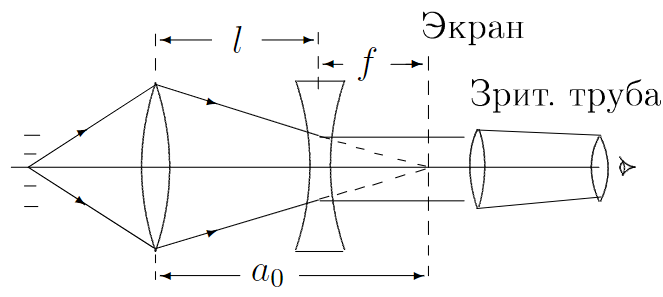
\includegraphics[width=10cm]{фокусное_рассеивающей.png}
        \caption{ Определение фокусного расстояния рассеивающей линзы}
        \label{focus} %% метка рисунка для ссылки на него
        \end{center}
    \end{figure}
    \item Перемещая рассеивающую лизну, найдем в окуляре резкое изображение сетки.
    \item Расстояние между сибирающей линзой и экраном получилось $ a_0 = 39.2 см$
    \item Расстояние между линзами $ l = 30.4 \; см$
    \begin{equation}
        f = l - a_0  = 8.8 \; см
    \end{equation}
    \item  Перевернув линзу, повторим измерения $f = 8.0 \; см$.
\end{enumerate}

\subsection{Телескоп Кеплера}

\begin{enumerate}
    
\item Отбираем две собирающие линзы. В качестве коллиматора используем используем 3 -ю линзу. 
\item Определяем размер изображения h1 = 12 дел/мм ($h_1 = k\alpha_1$, где k - коэффициент характеризующий увеличение зрительной трубы, $\alpha_1 - угловой размер изображения$ ) 
\item Соберем модель телескоппа: за объектив берем линзу с максимальным фокусным расстоянием,  окуляр - расстоянии примерно равном сумме фокусных расстояний обеих линз телескопа. 
\item Слегка перемещая окуляр модели вдоль оптической скамьи, получаем изображение сетки. Расстояние между объективом и окуляром оказалось равным 38.8 см, что совпадает к суммой фокусных расстояний окуляра и объектива .
\item Рассчитаем увеличение:
\begin{equation}
   N_T = \frac{\alpha'}{\alpha} = \frac{f_1}{f_2} = \frac{D_1}{D_2}
\end{equation}
$N_T = 1,7$
\item Определим угловое увеличение телескопа $h_2 = k\alpha_2, \; здесь \;  \alpha_2 - угловой \;  размер \; изображения \;  деления \; через \; телескоп$
\\
$h_2 = 19 \frac{дел}{мм},\\ N_T = 1,6 $
\item Определим увеличение телескопа через отношение диаметров $D_1 \; и \; D_2$ - оправы объектива и изображения соответственно.
\\
$N_T = \frac{D_1}{D_2} = \frac{4,4}{3,1} = 1,4$ 
\\
$  N_T = \frac{\alpha'}{\alpha} = 1,4$ 
    
\end{enumerate}

\subsection{Труба Галилея}

\begin{enumerate}
    \item Не троная коллиматор и объектив, заменяем окулярную линзу рассеивающей на расстоянии равном разности фокусов объектива и окуляра.
    \item Рассчитаем увеличения
    
    \begin{table}[H]
        \centering
        \begin{center}
        \end{center}
        \vspace{0.1cm}
        \label{tab:my_label}
        \begin{tabular}{ |p{2cm}|p{2cm}|p{2cm}|p{2cm}|}
     \hline
      & $f_1 \backslash f_2$ & $h_2\backslash h_1$ & $D_1\backslash D_2$ \\
     \hline
     $N_T$ & 2,1 & 1,9 & 1,7 \\
    \hline
    \end{tabular}
    \caption{Увеличение трубы Галилея}
    \end{table}

\end{enumerate}

\subsection{Модель микроскопа}

\begin{enumerate}
    \item Берем самые короткофокусные линзы, для создания увеличения $N_M = 5$.
    \begin{figure}[H]
        \begin{center}
        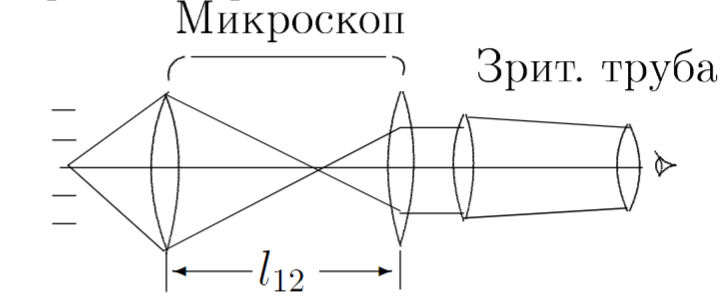
\includegraphics[width=8cm]{микроскоп.png}
        \caption{ Модель микроскопа}
        \label{micros} %% метка рисунка для ссылки на него
        \end{center}
    \end{figure}
    \item Рассчитаем необходимый интервал $\varDelta$ и длину тубуса $l_{12}$
    \begin{equation}
       N_M = N_1N_2 = -\frac{\varDelta}{f_1}\frac{L}{f_2}; \; \varDelta = l_{12} - f_1 - f_2, где \; L= 25см
    \end{equation}
    $\varDelta = 16,05 см$
    \\
    $l_{12} = 34,3 см$
    \item Фокусируем модель микроскопа на сетку осветителя, перемещая осветитель вдоль оптической скамьи до техпор, пока в окуляре не появится отчетливое изображение.
    \item Измерим величину изображения $h_2 = 26,5$.
    \item Рассчитаем увеличение по формуле:
    \begin{equation}
        N_M = - \frac{h_2}{h_1}\frac{L}{f} = 5,2 
    \end{equation}
    Полученное значение близко к ожидаемому.
\end{enumerate}

\subsection{Оценка птогрешностей}

Так как погрешность в данной работе связана не только с ценой деления инструмента (линейки), но и с определением наиболее четкого изображения, поэтому будем считать погрешность прямых измерений равной $\sigma = 0.5 см$.
\\ 
Погрешность для измерения фокусного расстояния рассеивающей линзы:
\begin{equation}
    \sigma_f = \frac{2\cdot0.5}{30.4+39.2}\cdot 8.8 = 0.1 \; см
\end{equation}
\\
\textbf{Погрешность для рассчета увеличения трубы Кеплера}
\begin{enumerate}
    \item через фокусные расстояния/диаметр оправы объектива
    $\sigma_N = \sqrt{\sigma^2_{f_1/D_1}+\sigma^2_{f_2/D_2}} = 0.7$
    \item Погрешность измерения углового увеличения составляет полделения.
    $\sigma_N = \sqrt{\sigma^2_{h_1}+\sigma^2_{h_2}} = 0.4$
\end{enumerate}
\par

\textbf{Погрешности для трубы Галилея.}
\begin{enumerate}
    \item через фокусные расстояния/диаметр оправы объектива
    $\sigma_N = \sqrt{\sigma^2_{f_1/D_1}+\sigma^2_{f_2/D_2}} = 0.5$
    \item Погрешность измерения углового увеличения составляет полделения.
    $\sigma_N = \sqrt{\sigma^2_{h_1}+\sigma^2_{h_2}} = 0.4$
\end{enumerate}
    \par

\textbf{Погрешности для измерений микроскопа}:
\begin{enumerate}
    \item     $\sigma_\varDelta = \frac{0.5*3}{34.3+7.5+10.7} \cdot 16.05 = 0.3 см$
    \item $\sigma_N = \sqrt{\sigma^2_{f_1}+\sigma^2_{f_2}+\sigma^2_\varDelta} = 0.8$
    \item $\sigma_N = \sqrt{\sigma^2_{h_1}+\sigma^2_{h_2}+\sigma^2_f} = 0.5$
\end{enumerate}

Значения измерений хорошо сходятся в пределах погрешностей.
\subsection{Вывод}
В ходе работы были определены фокусные расстояния собирающих и рассеивающей линзы. Из этих линз сконструировали оптические приборы: труба Кеплера, труба Галилея и микроскоп. 
Определили их увеличения различными способами.
\newpage

\end{document}